\documentclass[12pt]{article}

% to compile: PDFLaTeX -> BibTeX -> PDFLaTeX -> PDFLaTeX -> View PDF
% in this way both the table of content and bibliography is created correctly
% shortcutkeys in TexMaker is F6 -> F11 -> F6 -> F6 -> F7

\usepackage[english]{babel} % Forklarer at dokumentet er dansk
\usepackage[latin1]{inputenc} % Forklarer hvilket charset er dokumentet skrevet i
\usepackage{graphicx} % Manage external pictures
\usepackage{pdfpages} % This package simplifies the insertion of external multi-page PDF or PS documents.
\usepackage{listings} % to insert programming code within the document. Many languages are supported and the output can be customized.
\usepackage{float} % Bruges blandt andet til H i figures
\usepackage{fancyhdr} % change header and footer of any page of the document.
\usepackage[pdfborder={0 0 0 0}]{hyperref} % Indstter url-adresser og ref-links korrekt. Disse kan vises som url adressen eller bare tekst og er klik-bare i pdf dokumentet. \href{URL}{text}
\usepackage{verbatim} % improves the verbatim environment
\usepackage{rotating} % Bruges til at vende teksten vertikalt
\usepackage{framed} % Benyttes til at lave bokse om diverse ting.
\usepackage{multirow} % Benyttes til avancerede tabeller
\usepackage{amssymb} % it adds new symbols in to be used in math mode.
\usepackage{color} % it adds support for colored text
\usepackage{natbib} % gives additional citation options and styles
\usepackage{subfigure} % addfunctionality for subfigures

\usepackage{tikz}
\usepackage[none]{hyphenat}

% All of this crap is used for the parsing table DO NOT DELETE!
\def\inputGnumericTable{} 
\usepackage{array}
\usepackage{longtable}
\usepackage{calc}
\usepackage{multirow}
\usepackage{hhline}
\usepackage{ifthen}
% End of parsing table crap

%added inorder to make pipe literals withinb tables in the ebnf
\usepackage[T1]{fontenc}

\lstset{
	language=java,
	keywordstyle=\bfseries\ttfamily\color[rgb]{0,0,1},
	identifierstyle=\ttfamily,
	commentstyle=\color[rgb]{0.133,0.545,0.133},
	stringstyle=\ttfamily\color[rgb]{0.627,0.126,0.941},
	showstringspaces=false,
	basicstyle=\small,
	numberstyle=\footnotesize,
	numbers=left,
	stepnumber=1,
	numbersep=10pt,
	tabsize=2,
	breaklines=true,
	prebreak = \raisebox{0ex}[0ex][0ex]{\ensuremath{\hookleftarrow}},
	breakatwhitespace=false,
	aboveskip={1.5\baselineskip},
	frameround=fftt,
	frame=shadowbox,
	columns=fixed,
	upquote=true,
	extendedchars=true,
	breaklines=true
%	alsoletter={'},
%	morekeywords={'}
% frame=single,
% backgroundcolor=\color{lbcolor},
}
\newcommand\XOR{\mathbin{\char`\^}}
\usepackage{textcomp}


% We want to use fancyhdr this time.

\begin{document}

%\includepdf{./titelblad/titelblad.pdf}

%\setcounter s�tter hvilket level i depth tableofcontents skal vise til, default er 3: alts� subsubsection. 
%Level -1: \part, 0: \chapter, 1: \section, 2: \subsection, 3: \subsubsection, 4: \paragraph*
%\setcounter{tocdepth}{3}

\begin{center}

\rule{\textwidth}{3pt}\\
\hrulefill\\
{ \huge \bfseries Preface} \\
\hrulefill\\
\rule{\textwidth}{3pt}\\
\end{center}

Denne rapport er skrevet af Bjarke Carstens, Andreas N�rskov og Stephan Grooss. Nedenunden findes underskrifter samt hvem der har bidraget til hvilke dele af rapporten.

\vspace{10 mm}

\begin{center}
\begin{minipage}{6cm}
\begin{center}
\makebox[5cm]{\hrulefill}\\
Bjarke Carstens\\
\makebox[5cm]{}
\makebox[5cm]{}
\makebox[5cm]{\hrulefill}\\
Andreas N�rskov\\

\end{center}
\end{minipage}
\begin{minipage}{6cm}
\begin{center}
\makebox[5cm]{\hrulefill}\\
Stephan Grooss\\
\end{center}
\end{minipage}

\vfill
{\large \today}

\end{center}




\newpage

\tableofcontents

\newpage
\part{Introduction}
\section*{Introduction}

\part{Virksomhedsbes�g}
aeggaegaeeagjndztgosgnlgnlkjgsdfrl. \\
\subsection{?}
\input{?}

\begin{itemize}
\item
\item
\begin{itemize}
\item
\item
\end{itemize}
 

\end{itemize}
%aeggaegaeeagjndztgosgnlgnlkjgsdfrl. \\
\subsection{?}
\input{?}

\begin{itemize}
\item
\item
\begin{itemize}
\item
\item
\end{itemize}
 

\end{itemize}

\part{Process teori}
\subsection*{Extreme Programming}
Extreme programming er en agil udviklingsmetoder der kom frem i starten af 90'erne og var opfundet af en mand ved navn Kent Beck. Metoden best�r af et netv�rk af v�rdier og praktikker som bygger p� sund fornuft.
Mange firmaer l�gger deres programeringsprocess om til agile udviklingsmetoder. Tit bliver det en blanding mellem de mere plandrevne og agile processer da ikke alle kunder f�ler sig sikrer ved at bruge en ren agil metode som xp eller scrum. I andre tilf�lde kan man ogs� bruge praktikker fra plandrevne metoder hvis programm�rerne skal opn� enighed om design af programmet. Her kan man bruge diagrammer som don�nemodeller, databasediagrammer osv.\\
For at extreme programming kan h�nge sammen har Kent Beck opsat 13 praktikker der skal sikrer at tidsrammen bliver overholdt og at programmet er kvalitetssikret. \\

\begin{itemize}
	\item Planning Poker (Kunden definerer prioritet)
	\item kort tid mellem realeses (Hurtig produktion)
	\item Metafor (F�lles termonologi og begreber)
	\item Simpelt Design (Opst�r l�bende, kun d�kke aktuelle behov)
	\item Definer Test First (Derefter kodes)
	\item Refactoring (Forbedre design l�bende)
	\item Par Programmering (2 udviklerer, 1 tastatur)
	\item Kollektivt Ejerskab (Enhver kan �ndre hvad som helst)
	\item L�bende Integration (Kompilering dagligt)
	\item 37 Timers Arbejdsuge (Dedikerede programm�rer, tr�thed medf�re fejl)
	\item Kundeinvolvering (Kunden stiller kravene)
	\item Kode Standard (Underst�tter de andre praktikker)
\end{itemize}

\subsubsection*{Personer og Roller}
Ligesom i plandrevne udviklingsmetoder er der forskellige personer der varetager forskellige roller/funktioner. Disse vil jeg liste herunder.\\

\textbf{Kunde/interesser}\\
Kunden definerer opgaver/userstories som er sm� stykker funktionalitet som programmet skal indeholde. Dette foreg�r i t�t relation til kunden(mund til mund).\\
Kunden estimerer prioriteringen af forskellige opgaver alt efter hvilken funktionalitet kunden mener er vigtigst.\\
Kunden er med til hvert realese for at se hvilke funktionaliteter kodeholdet har udvilket.\\
Kunden definerer om en accepttest er opn�et.\\

\textbf{udviklingteam}\\
Udviklingsteamet estimerer de forskellige userstories efter storypoints eller mandetimer.\\
Udviklingsteamet programmerer programmet ud fra userstories og sikrer kvalitet ved at bruge test first, par programmering og accepttests.\\

\subsubsection*{Proces}
Selve processen starter med at udviklingsteamet s�tter sig ned med kunden og snakker om hvilke funktionaliteter kunden �nsker i deres program. Sammentidig nedskriver udviklingsteamet disse funktionalitet ned p� en userstory som definere hvem der vil bruge denne funktionalitet, hvad den skulle kunne og hvad brugeren skal kunne f� ud af funktionaliten. Derefter skrives en accepttest p� bagsiden af userstorien som definere hvorn�r userstorien er kan s�ttes fra verify over p� done. Det kan v�re at udviklingstemaet bliver n�dt til at lave nogle ekstra userstories hvis noget teknologi er ukendt. Dette kaldes spikes.\\
N�r alle userstories er skrevet s�tter udviklingsteamet sig ned og begynder at estimerer hvor lang tid de enkelte userstories tager i storypoints. Det er her planning poker kommer ind i billedet. Hver enkelt medlem er udviklingsteamet f�r et s�t kort med fibonacci numrene 1/2, 1, 2, 3, 5, 8, 13, 20, 40, 100, ?, og en kaffekop. Man begynder spillet med at finde den userstory men mener tager gennemsnitlig tid at lave og tildeler den v�rdien 5. Ud fra denne story byder de forskellige udviklingmedlemmer ind p� hvad de mener de enkelte stories burde have i v�rdi med planningpoker kortene. kortene ? betyder at man ikke har nogen ide om hvor langt tid det tager at lave denne usertory og kaffekoppen at man skal holde en kaffepause. Dette kan v�re aktuelt hvis der er uenighed mellem udviklingsmedlemmerne. F�r en userstory 20 point eller mere er dette et tegn p� at userstorien er for stor. Den skal derfor deles op og de nye enkelte userstories skal godkendes af kunden og gives point igen.\\
N�r alle userstories er defineret udregnes udviklingsteamets velocity, som er det antal storypoint udviklingstemaet kan n� i en iteration. I XP kan en iteration v�re mellem 1-2 uger. N�r velocytien er fundet tegnes den ind p� et burndowndiagram, hvor man har antal storypoint op ad y-aksen og antal mandedage hen a x-aksen.\\
Derefter indvolveres kunden igen for at lave en proritering af de enkelte userstories for at finde ud af hvilke funktionaliteter der skal laves i den f�rste iteration. N�ar der er kunden har fundet ud af hvilke userstories han vil have lavet definerer udviklingsteamet tasks som s�ttes p� de enkelte userstories. Tasks er opgaver set fra udviklernes �jne og skal skrives som programeringsopgaver. Det kan f.eks. v�re skriv unittest, lav modelklasse til kunde, ops�t database med kundetabel osv.\\
Inden man begynder p� iteration 1 Har man oftes en iteration 0. Det er her udviklingsteamet s�tter udviklingmilj� op, definere kodestandarder, s�tter versionsstyring op osv. N�r dette er gjort kan udviklingsteamet g� igang med iteration 1. Her begynder udviklingteamet at programmerer i par. Hver dag holdes et kort stand-up meeting p� 10-15min hvor de enkelte medlemmer diskuterer hvor langt de er n�et og ser p� hvilke tasks der skal laves i l�bet af dagen. Sammentidig tegnes der ned p� burndown for at se om de har n�et at br�nde det antal storypoint der skal br�ndes. Man holder dette stand-up meeting for at der ikke skal diskuteres i l�bet af dagen, s� hver enkelt programm�r ikke spilder tid p� diskussion. Kan udviklingsteamet se p� deres burndown at de ikke kan n� iterationens opgaver bringes kunden ind for at se p� hvilken/hvilke userstories der kan pilles ud af iterationen. Sker dette tegnes en lige streg ned p� burndown for at illustrerer dette. N�r iterationen er f�rdig holdes et retrospektive hvor man ser p� hvad der gik godt og hvad der kunne v�re gjort bedre til n�ste iteration. Derefter gentages processen igen.\\
Efter nogle iterationer er passeret holdes der et realese som er atalt med kunden p� forh�nd, hvor udviklingsteamet holder en pr�sentation foran kunden/interesser, hvor de viser hvilke funktionaliteter de har lavet. Her vuderer kunden om han er tilfreds med programmet som det er nu eller om der skal arbejde viderer.

\textbf{udregning af velocity}
S�dan udregnes teamet velocity:
\begin{itemize}
 \item Kig p� storien af middel sv�rhedsgrad = "5" storypoint.
 \item Vurder hvor mange mandedage der skal bruges p� storien f.eks. 10.
 \item Velocity = 5/10 = 0,5 storypoints per mandedag.
 \item Antal storypoint teamet kan n� at lave i en iteration af 5 dage med 4 mand = 20*0,5 = 10
 \item Korriger for par programmering?
 \item Korriger for evt. sygdom og andet? (fokusfaktor)
\end{itemize}

\textbf{Kvalitetssikring}
udviklingstemaet kvalitetssikre koden p� flere m�der. Ved at sidde 2 ved et tastatur(par programmering). Det er ikke meningen at personen bagved skal afbryde ham der programmeres flow men komme med indskydende bem�rkninger hvis han er ved at lave fejl. Undervejs bytter de to programmerer og der byttes ogs� mellem de forskellige parprogrameringshold for at sikrer kodeejerskab. Dette giver ogs� kvalitetssikring da der er flere �jne p� den samme kode.
Test First som betyder at inden man laver en metode skirver man en unit test som tester om metoden fungerer korrekt. S� fejler testen er metoden ikke skrevet korrekt. Accepttests inden en opgave kan s�ttes over p� done skal den verificeres af en anden programm�r. Opfylder tasken accepttesten kan den s�ttes over p� done.


\subsection*{Scrum}
Scrum ligner p� mange m�der XP og de to agile planl�gningsmetoder har ogs� l�nt af hinanden. f.eks. kommer XP's stand-up meeting fra scrum. I scrum hedder dette Scrum meeting. \\
Scrum blev udviklet i 90'erne af en mand ved navn Ken Schwaber. Han brugte hvad der nu er kendt som scrum i hans firma. F�rst i 2001 udgav han bogen Advanced Development Methods sammen med Mike Beedle hvor de beskrev udviklingsmetoden. Mange firma har senere hen implementeret denne metode i deres projekter.\\

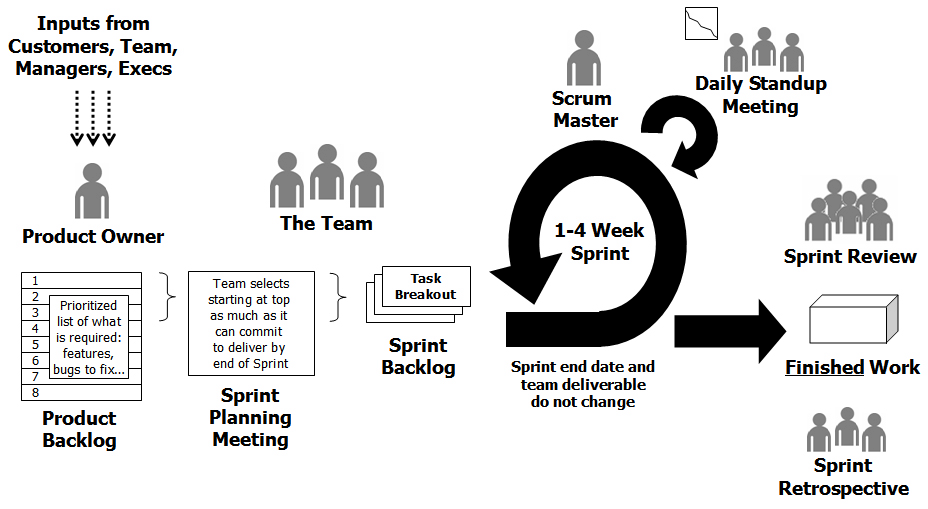
\includegraphics[scale=0.35]{includes/billeder/Scrumteam.png}\\

Her ses en model over de forskellige act�rer i et SCRUM team. 

\subsubsection*{Personer og Roller}
\textbf{Kunde/interesser}\\
Kunden/interesser er de/den person/personer der �nsker at f� udviklet et stykke software. I SCRUM har kunden ikke direkte kontakt med udviklingsteamet, men formidler istedet deres �nsker igennem product owner.\\

\textbf{Productowner}
Product owner er et mellemled mellem udviklingsteamet og kunden/interesser. Han st�r for at aftale med kunden hvilke funktionaliteter kunden �nsker at f� udviklet i deres program. Disse funktionaliter bliver skrevet ned i en productbacklog som p� mange m�der er userstories skrevet ned i listeform p� et stykke papir.\\

\textbf{Scrum Master}
Scrum Master fungerer som et mellemled mellem Udviklingsteamet og productowner. Han er en form for projectleder som er ansvarlig for scrumprocessen. Han leder de daglige scrum m�der og fungerer som en slags firewall, der fjerner hindringer for udviklingteamet. Scrum master kan godt v�re en del af udviklingsteamet.
\textbf{Udviklingsteam}
Et scrum udviklingsteam best�r typisk er et team p� 7-9 personer der alle er Analyserer, designer, tester, estimerer, planl�gger og f�lger op. Teamet er selvorganiseret og finder derfor selv ud af hvordan de vil arbejde.

\subsubsection*{Hvad er anderledes fra XP}


\subsection*{Kanban}
Kanban er en Udviklingsmetode udviklet af japserer og er totalt ubrugeligt.

\newpage

\part{Ideudvikling}
\section*{Navn p� Mobil App}
Food4Thought

\subsection*{Features}
\begin{itemize}
\item Hovedmenu
\item Food map
\item Opskriftliste og indk�bsliste
\item Personlige pr�ferencer (pris, tilberedningstid)
\end{itemize}

\subsection*{Ekstra features}
\begin{itemize}
\item Brugerpr�ferencer (Kalorie, protein, fedt indhold)
\item Forslag til hvor tingene kan k�bes og hvor de kan findes i butikken
\item GPS som finder det n�rmeste supermarked med varerne p� indk�bslisten (vis kun supermarkeder der samarbejdes med)
\end{itemize}


\section{Statement p� Mobil App}
Food4Thought er en app som sparer dig tid p� at finde ud af hvad du skal have at spise, hvilke ingredienser du skal bruge og hvordan det skal tilberedes. 

\section{M�lgruppe}
Unge mennesker der ikke har tid til at finde og sammens�tte deres m�ltider, som gerne vil have hj�lp til hurtigt vil kunne sammens�tte et m�ltid ud fra ingredienser de godt kan lide. \\

Midaldrende karriere mennesker som er p� arbejdsmarkedet og har en stresset hverdag, og har ikke n�dvendigvis tiden til at sammens�tte et m�ltid, til familien om aftenen. \\

Mennesker som mangler ny inspiration til retter, men s�ger en begr�nset metode til at finde nye opskrifter p�.

\section{Personas}
Thomas p� 25 er matematik studerende p� AAU og har derfor en meget travl hverdag. Han har ikke tid og overskud til madlavning n�r han kommer hjem og han ender tit med at spise pasta og fastfood. \\

Bettina er enlig mor med 3 b�rn p� 35. Hun er sygeplejerske p� Riget i K�benhavn og har derfor tit varierende vagter. Pga. Bettinas vagter har hun ikke meget tid til madlavning, hvilket resulterer i at hendes b�rn tit spiser takeaway. \\

Niels p� 32 er advokat, karriere menneske og har alt for travlt til at have overskud til madlavning. Han spiser ofte p� restaurant, hvilket koster kassen s� han har en interesse i at cutte lidt ned i sine udgifter, men ikke p� bekostning af at skulle bruge for meget tid p� det.  

\section{Brugs scenarier}
Thomas er p� vej ned til supermarkedet da hans mave rumler. Han er ikke for god til at lave mad eller til at k�be ind. F�r Thomas g�r ind i supermarkedet tager han sin mobil op ad lommen og starter programmet: Food4Thought. \\

Sk�rmbilledet p� Thomases mobil viser knapperne: "FoodMap", "Recipes", "shoppinglist", "Favorite" og "My Account". Han v�lger "FoodMap" og trykker p� knappen. \\

Et nyt sk�rmbillede fremvises hvor han kan indtaste sin favorit ingrediens i toppen. Thomas indtaster "chicken", hvorefter teksten fremvises i en bobel midt p� sk�rmen. \\

Omkring boblen fremst�r 6 andre bobler, som hver indeholder ingredienser Thomas kan v�lge skal indg� i hans opskrift. \\

Han v�lger "bulgur" og nye valgmuligheder popper frem. Men Thomas er ikke tilfreds med disse muligheder og trykker derfor p� boblen i midten for at blive pr�senteret for nye muligheder. \\

Thomas forts�tter med at v�lge ingredienser indtil han har valgt 5. De valgte ingredienser fremvises i en dialogboks nederst p� sk�rmen. Thomas trykker tilsidst p� knappen "To recipes", og et nyt sk�rmbillede fremvises med en tabel af forskellige opskrifter der indkludere korte beskrivelser samt billeder af retterne. Thomas v�lger en af retterne ved at trykke p� den. \\

Et nyt sk�rmbillede fremviser nu et stort billede af retten, tilberedningsmetoden, samt en indk�bsliste i bunden. \\

Thomas er nu ellevild, da han ikke havde forventet at kylling med pesto, mandler, bulgur og chili kunne smage s� godt. Han er begejstret over kun at have brugt 2 min p� at finde opskriften, samt 5 min p� at k�be ingredienser.

\newpage

\section{Prototyper}
Vi har valgt at lave prototyper til 3 af de vigtige sk�rmbilleder for appen: hovedmenu, foodmap og opskriftsforslag

\begin{figure}[H]
\begin{center}

\includegraphics[scale=0.85]{includes/billeder/hovedmenu.png}
\caption{hovedmenu}
\label{fig:ideudvikling:hovedmenu}
\end{center}
\end{figure}

\textsf{Hovedmenu:} ~\ref{fig:ideudvikling:hovedmenu} \\
Hovedmenuen er det f�rste sk�rmbillede brugeren bliver pr�senteret og giver mulighed for at navigerer rundt i de forskellige funktionaliteter i appen som food-map, recipelist, shopping list og favorites. \\

\begin{figure}[H]
\begin{center}
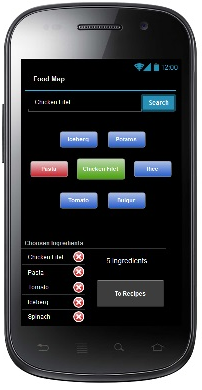
\includegraphics[scale=0.85]{includes/billeder/foodmap.png}
\caption{foodmap}
\label{fig:ideudvikling:foodmap}
\end{center}
\end{figure}

\textsf{Foodmap:} ~\ref{fig:ideudvikling:foodmap} \\
Foodmap er selve hoved funktionaliteten i programmet. N�r brugeren bliver m�dt af denne sk�rm kan de i �verste boks, skrive hvilken hoved ingrediens de �nsker i deres opskrift. N�r brugeren har skrevet en vare og trykket s�g, bliver den fremvist i midten af sk�rmen, omkring ingrediensen bliver der nu fremvist forskellige hoved kategorier af ingredienser.
Brugeren kan nu v�lge 3-5 ingredienser fra de valg muligheder der popper frem p� sk�rmen. Hver gang brugeren har valgt en ingrediens bliver den tilf�jet til en liste i nederste venstre hj�rne. Herfra kan brugeren ogs� slette sine valg. N�r brugeren er tilfreds med sine valg, kan han nu trykke videre til opskrifter. \\

\begin{figure}[H]
\begin{center}
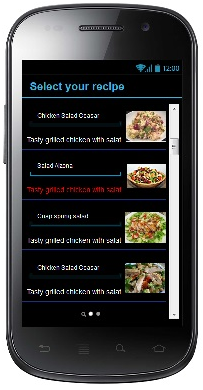
\includegraphics[scale=0.85]{includes/billeder/opskriftliste.png}
\caption{opskriftsforslag}
\label{fig:ideudvikling:opskriftsforslag}
\end{center}
\end{figure}

\textsf{Opskriftsforslag:} ~\ref{fig:ideudvikling:opskriftsforslag} \\
Opskrift forslags funktionen af programmet, fremkommer s� snart brugeren har lavet sin ingrediens liste. Brugeren bliver m�dt af forskellige opskrift forslag som matcher de s�gs kriterier der er fremsat. Alle opskrifter bliver fremvist med et billede, beskrivelse samt opskrift navn. Hver enkelt opskrift kan v�lges og �bnes i ny fane, de kan herefter gemmes hvis det �nskes. \\

\newpage

\section{Arkitektur}
Appen tilg�r en gratis tilg�ngelig API med over 200.000 opskrifter. \\
Arkitektur afsnittet omhandler hvor vi ligger databasen; lokalt eller p� server? Hvordan og hvor ofte vi opdaterer den?

\includegraphics[scale=0.40]{includes/billeder/arkitektur.png}
% skriv beskrivelse

\newpage

\section{Business Canvas}
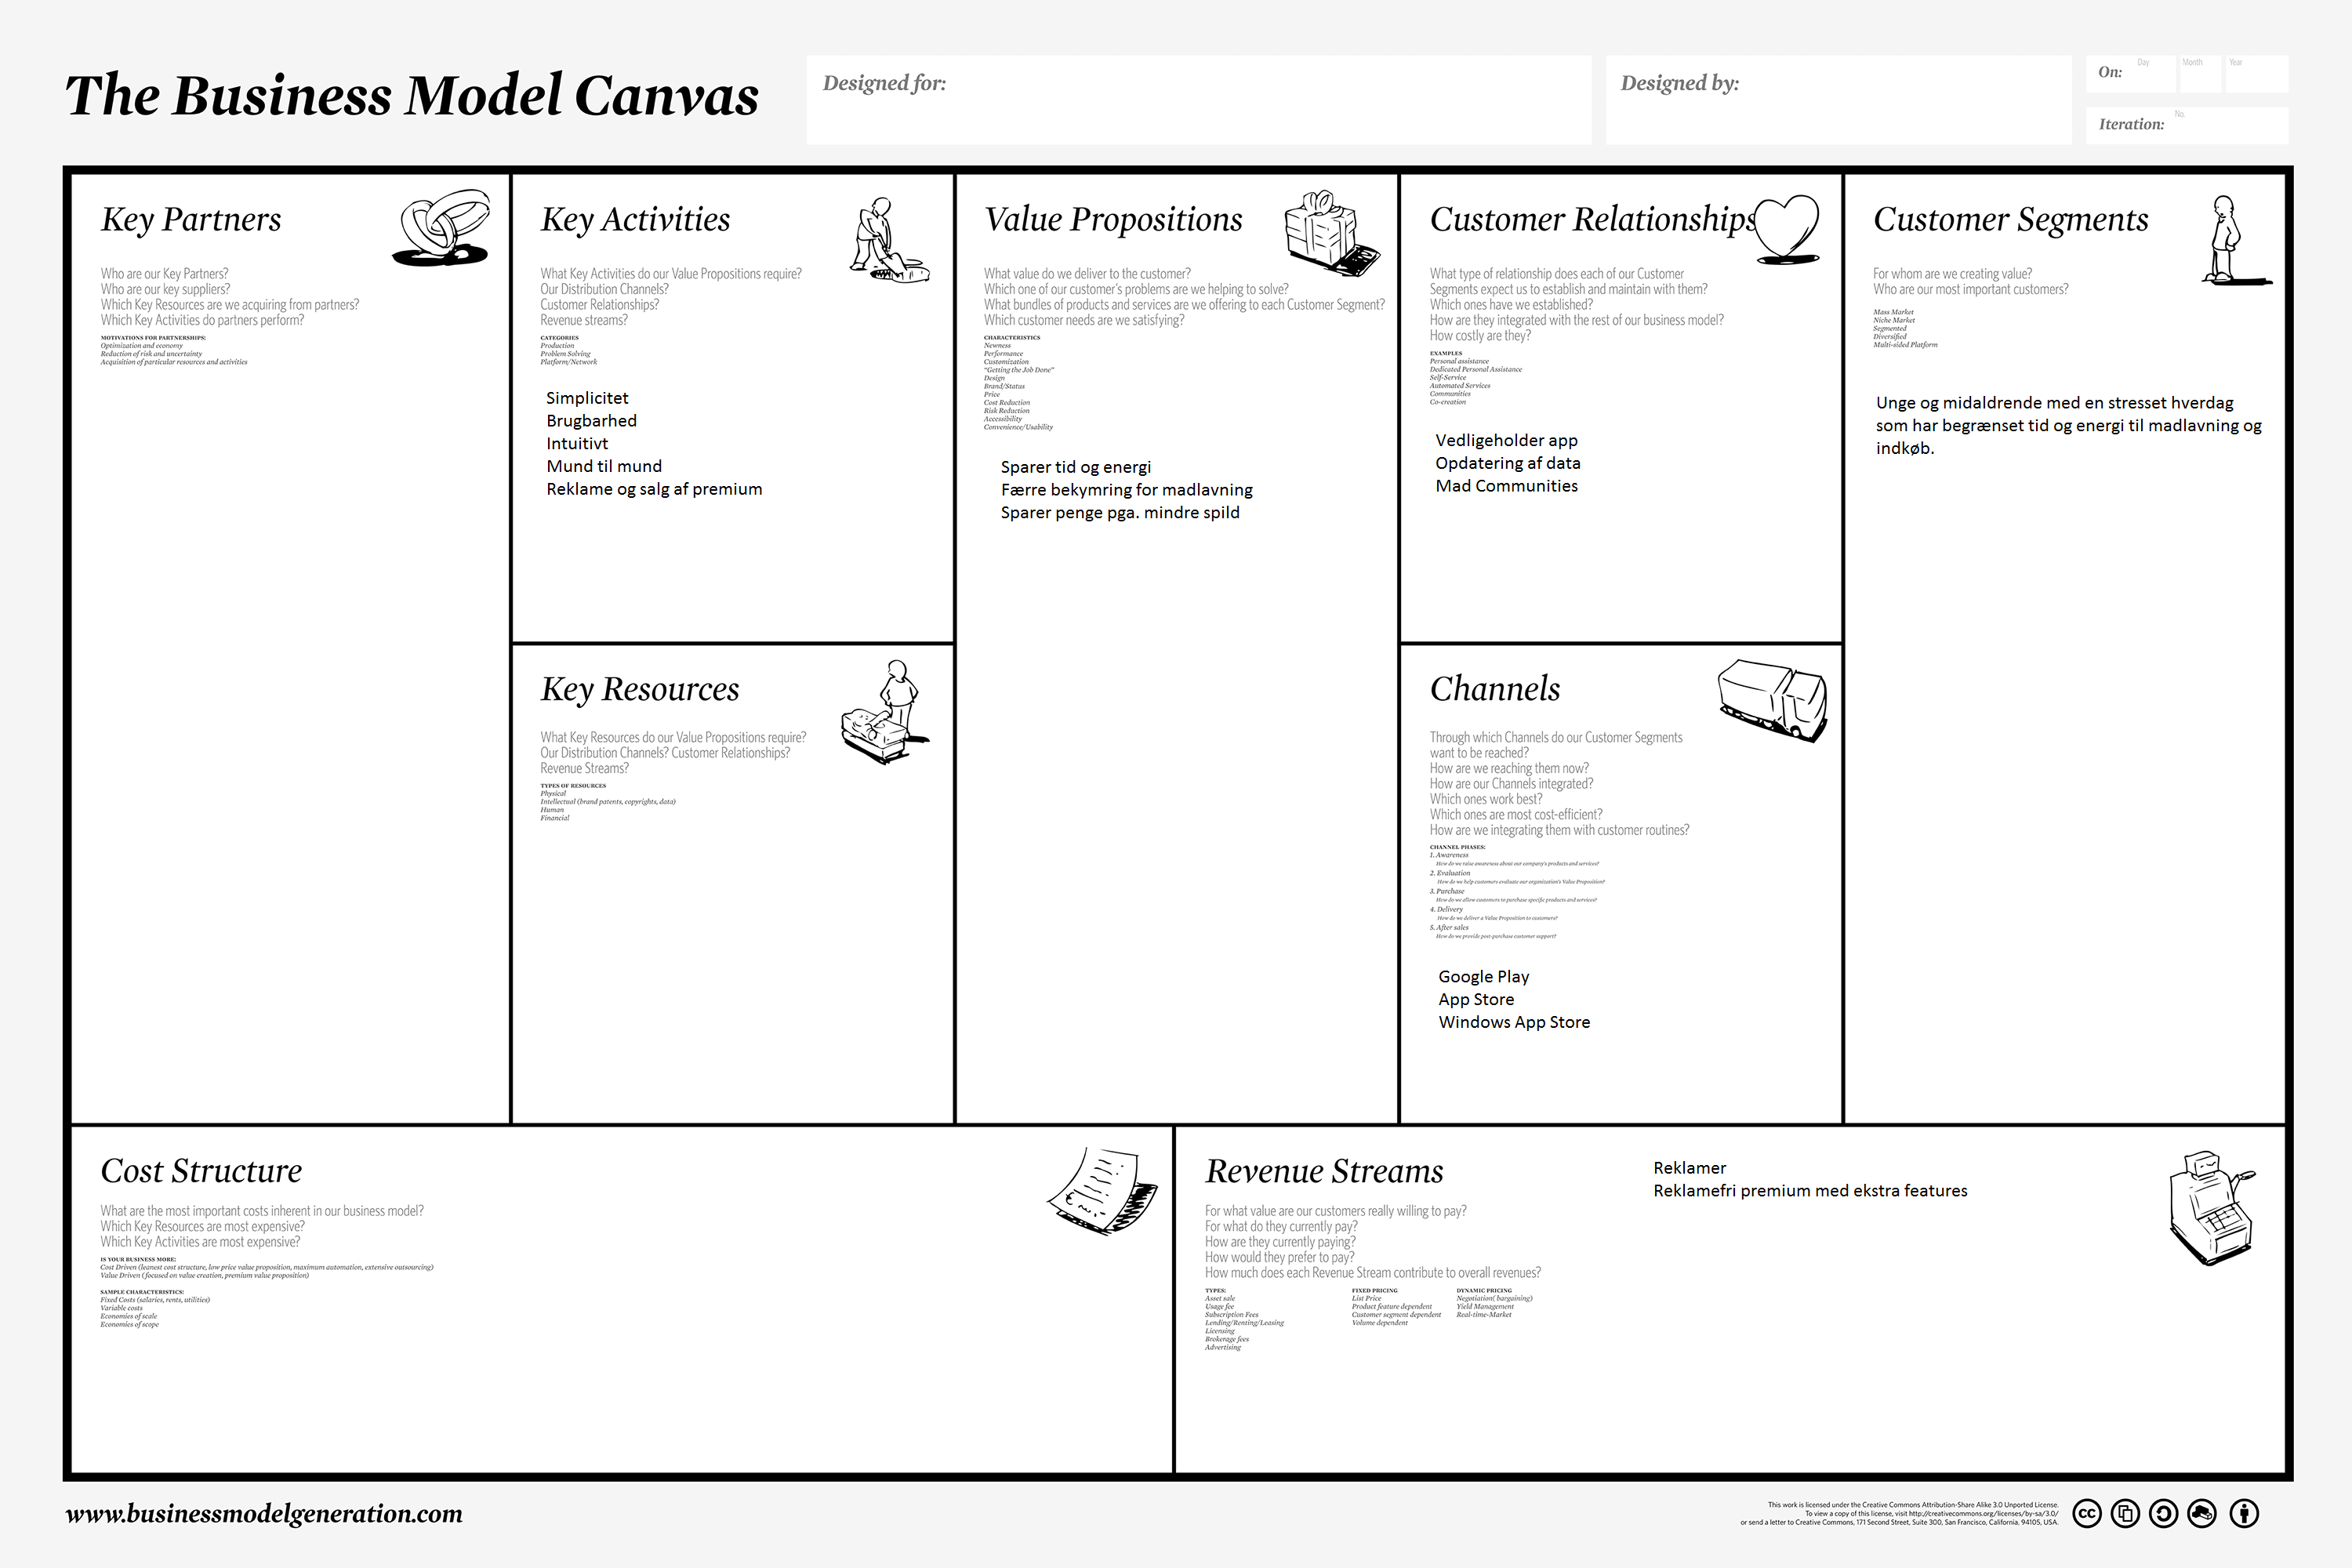
\includegraphics[scale=0.18]{includes/billeder/business_model_canvas.png}

\subsection{Key Activities}
\textsc{N�gle v�rdier:} \\
N�gle v�rdierne for vores ide er simplicitet, brugbarhed og intuitiv; appen skal v�re simpel at bruge, nem at l�re og skal give brugeren et hurtigt relevant resultat. \\

\textsc{Hvordan spreder vi produktet:} \\
Vi vil sprede produktet via mund til mund, som skal motiveres at brugerne synes om vores app. \\

\subsection{Value Propositions}
Appen skal gerne spare brugerne tid og penge ved at de bruger mindre tid p� at planl�gge madlavning, samt at brugerne gerne skulle f� mindre madspild ved at undg� impulsshopping. Dette skal helst ogs� betyde er der er f�rre bekymringer med madlavning. \\

\subsection{Customer Relationships}
Vores kundeforhold inkludere at vi s�rger for at vedligeholde appen ved blandt andet l�bende at opdatere og tilf�je nye opskrifter. Dette kan evt. g�res i samarbejde med online mad f�llesskaber.


\subsection{Customer Segments}
Vores kundesegmenter vil v�re unge og middelaldrende med en stresset hverdag, som har begr�nset tid og energi til at deres daglige madlavning og indk�b.

\subsection{Channels}
Vi vil tilbyde appen til vores kunder gennem de typsike app stores: Google Play, App Store og Windows App Store afh�ngigt af teknologien.

\subsection{Cost structure}
Vores omkostninger er i f�rste omgang den tid vi som udviklere ligger i udviklingen af appen, samt at hvis vi beslutter at benytte en API som database adgang vil dette give lidt l�bende omkostninger.

\subsection{Revenue Streams}
Vores plan for at tjene penge p� appen er gennem reklamer og reklamefri premium app med ekstra funktionalitet.

\subsection{Muligheder for tilpasning af business canvas og ide}
Vi har gode muligheder for at tilpasse business canvases til at ramme en anden m�lgruppe som fx diabetikere eller fitness interesserede ved at lave f� �ndringer p� key partners, cost structure og customer segments. I appen kan vi i nogle tilf�lde n�jes med at tilpasse vores database efter det specifikke kunde segment.

\section{Vision}
\textsf{Food4Thought:} \\
Food4Thought er en app til folk som, i deres hverdag, har for travlt til at bruge en masse tid p� planl�gning af indk�b, samt forberedelse af madlavning. I mods�tning til andre apps, hjemmesider og s�gemaskiner tilbyder Food4Though en simpel, intuitiv og effektiv brugergr�nseflade til hurtigt og elegant at give brugeren forslag til ingredienser, opskrifter med instruktioner og en indk�bsliste.

\newpage

\section*{Kvalitetssikring}
\subsection{Kvalitetsscenarier}
Her er de forskellige kvalitetsscenarier vi forventer kan have relevans for systemet. \\

\begin{figure}[H]
\begin{center}
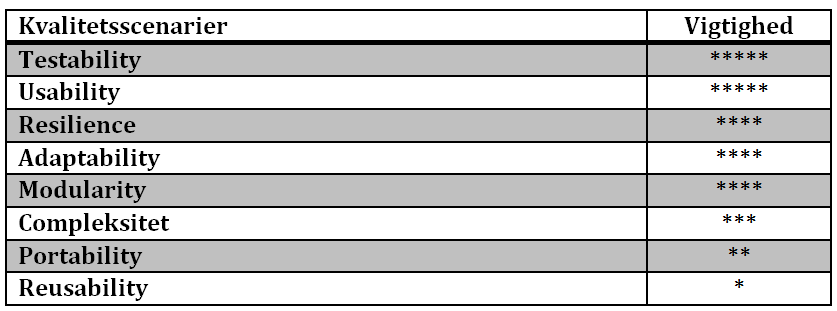
\includegraphics[scale=0.60]{includes/billeder/kvalitetsscenarietabel.png}
\caption{Kvalitetsscenarier}
\end{center}
\end{figure}

\textsf{Termer:} \\

Testability/testbart: \\
Funktionaliteten for skal v�re testbar for at kunne sikre usability. \\

Usability/brugbarhed: \\
Appen skal v�re nem at bruge for at den adskiller sig fra andre apps indenfor markedet. \\

Resilience/modstandsdygtigt: \\
Systemet skal kunne komme op at k�re hurtigt igen efter problemer. \\

Adaptability/tilpasseligt: \\
Systemet skal nemt kunne tilpasses i forhold til udvikling af nyt system eller krav�ndringer. \\

Modularity/modul�rt:\\ 
Det er vigtigt at systemet er modul�rt for at sikre adaptability og scalability.\\

Complexity/komplekst: \\
For at appen kan blive tilpas nem at bruge og adskille sig fra andre lignende apps er kompleksitet er n�dvendighed is�r i forhold til FoodMappet samt eventuelle algoritmer til at give brugeren relevante forslag til ingredienser og opskrifter. \\

Portability/overf�rlighed:\\ 
P� l�ngere sigt er det vigtigt at appen kan portes til andre platforme, men i f�rste omgang vil det v�re en fordel at fokusere p� en enkelt platform for at skabe en vis interesse for appen f�rst. S� kan man begynde at bruge resurser p� at porte den n�r den har vist sig at have potentiale. \\

Reusability/genbrugelighed: \\
Det er p� l�ngere sigt vigtigt at appen kan genbruges til videre udvikling fx som: diabetiker eller fitness app. \\
Samt at det ogs� vil v�re en fordel at kunne genbruge databasen til p� platforme. \\

Reliability/p�lidelighed: \\
Hvis vi havde valgt at fokusere p� en diabetiker version af appen ville det v�re meget vigtigt at brugeren kan stole p� informationen. \\

Robustness/robust: \\
Det er ikke s� vildt vigtigt at appen ikke crasher idet at den blot kan startes igen.
Dog er det vigtigt at server databaserne kan h�ndtere et vist antal foresp�rgsler n�r der opdateres med nye opskrifter. \\


\newpage

\subsection{Kravscenerier}
Vi har lavet kravscenerier til de 2 vigtigste stories: "Bruger vil gerne have ingrediens forslag" og "Bruger vil gerne have liste med opskrifter". \\  

\textbf{Bruger vil gerne have ingrediens forslag} \\
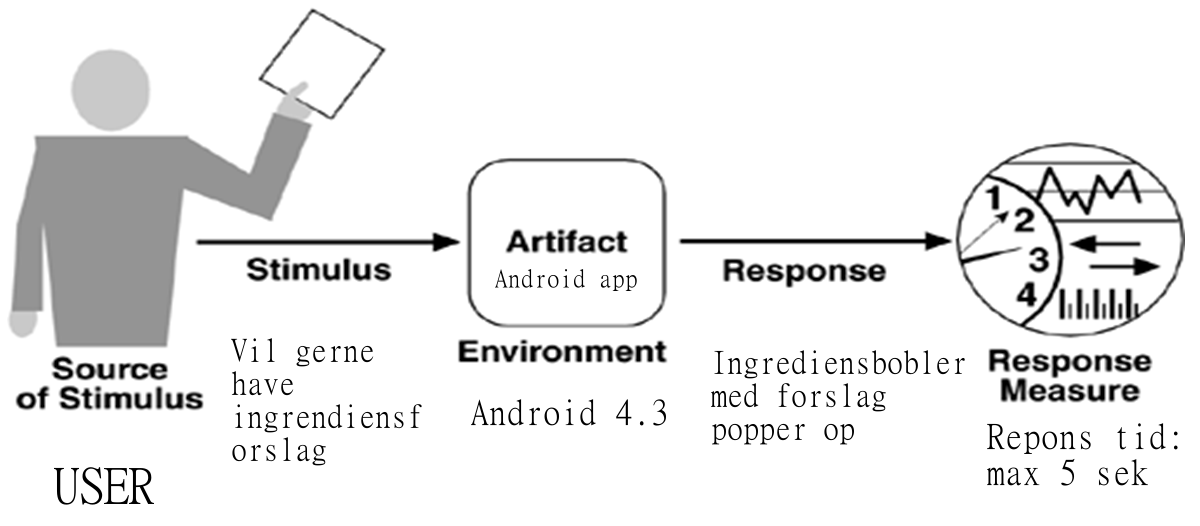
\includegraphics[scale=0.30]{includes/billeder/kravsscenerie_foodwheel.png} \\ \\
I dette scenarie vil brugeren gerne have forslag til ingredienser. Han interagerer s� med genstanden som er en android app i milj�et Android 4.3 og f�r som respons vist grafiske bobler der indeholder forslag til ingredienser indenfor maks 5 sekunder. Den korte responstid er vigtig for at brugeren f�r en god oplevelser og ikke bliver ut�lmodig.

\textbf{Bruger vil gerne have liste med opskrifter} \\
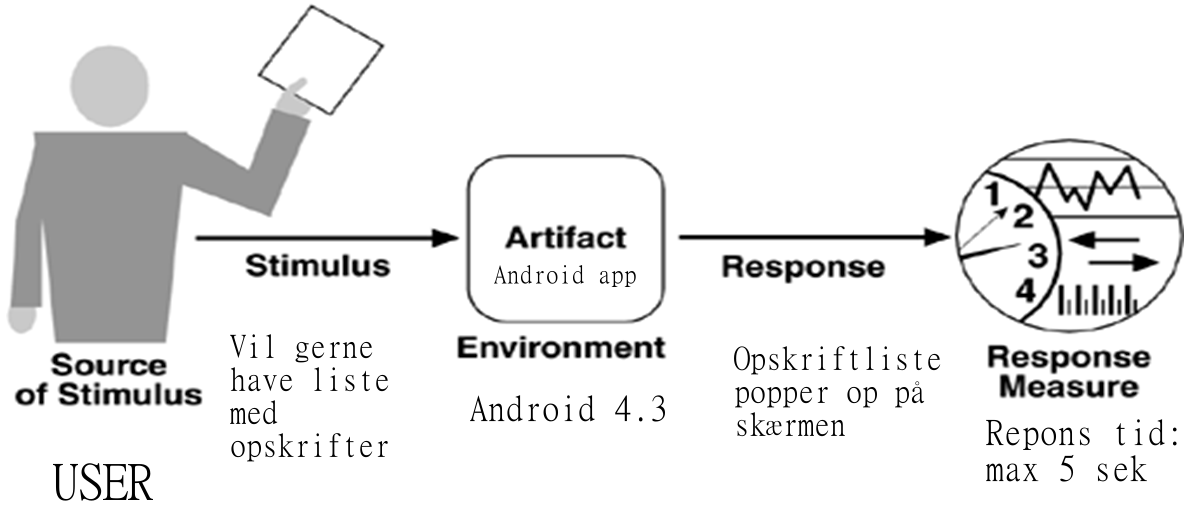
\includegraphics[scale=0.30]{includes/billeder/kravsscenerie_opskriftliste.png} \\ \\
I dette scenarie vil brugeren gerne have en liste med forslag til opskrifter. Han interagerer s� med genstanden som er en android app i milj�et Android 4.3 og f�r som respons vist en liste af opskrifter indenfor maks 5 sekunder. Den korte responstid er vigtig for at brugeren f�r en god oplevelser og ikke bliver ut�lmodig.

\newpage

\part{Projekt planl�gning}
\section*{Planl�gning og styring}
Til planl�gning og styring benytter vi iterationsplan med userstories og tasks samt en releaseplan og et burndown chart. \\
Vi har brugt scrum master for alle sprints, hvilket Bjarke har st�et for. Dette gjorde vi selv i sprint 1 som egentligt var baseret p� xp, men valgte at g�re det fordi det gav mening. Vi har valgt ikke at have en product owner idet at det ikke virkede effektivt i s� lille en gruppe og det giver ikke mening at productowner er en del af udviklingsteamet, da han dermed bliver mere tilb�jelig til at godkende �ndringer. Accepttest har vi skrevet bag p� vores userstories, hvor vi s� for at godkende dem har haft en af gruppemedlemmerne til at tjekke at det er er opfyldt, samt at koden for den bestemte funktionalitet har kunnet kompileres og eksekveres uden at g� ned.

\subsection*{Teknologi beslutninger}
Versionsstyring: GIT \\
Teknologi: Android og SQLite \\ 
Rapport skrivning: LaTex \\
IDE: Eclipse

\subsection*{Kvalitetssikring og test}
Vi har benyttet par programmering i det omfang det ellers har givet mening. \\
I det f�rste 3 sprints har vi valgt ikke at benytte unit testing da vi, p� grund af teknologien, er pressede tidsm�ssigt til at have funktionalitet f�rdigt til produkt reviews. \\ 
Automatisk l�bende integration og test ville blive for tidskr�vende at s�tte op, men pusher ofte via GIT efter at have sikret at det kan kompileres og eksekveres.

\newpage

\subsection*{Velocity}
Vi forventer at have 4 timer om dagen per mand i gruppen. Dvs. 8 mandetimer om dagen med 2 hold. \\
4 dage f�rste uge. \\
4 dage anden uge. \\
3 dage tredje uge. \\

5 storypoint (standard) tager 8 mandetimer \\
5/8 = 0,625 storypoint per mandetime \\

%dette skal �ndres...
40 mande timer i en iteration
40*0,625 = 25 storypoints per uge
			5 storypoints per dag \\

4 sprints i alt.

\subsection*{Revurderet Velocity}
F�lgende har vi fundet ud af vores velocity er lavere pga. manglende erfaring og teknisk niveau for nogle i gruppen.
Dette resulterer i at vi ikke helt har resourcerne for to hold men n�rmere 1,5.\\

Vi forventer at have 4 timer om dagen per mand i gruppen. Dvs. 6 mandetimer om dagen med 1,5 hold.\\

24 mande timer i en iteration\\
24*0,625 = 15 storypoints per uge\\
			3,75 storypoints per dag \\

\newpage

\section*{Sprint 0}
Sprint 0 benyttede vi til at lave produktbacklog, iterationsplan og burndown. Samt at lave spike p� interfacet til foodmappet. \\
Vi skulle ogs� have lavet spike p� database men n�ede det ikke. \\ 
I �vrigt var Bjarke var ikke tilstede hverken onsdag, torsdag og fredag pga. Gr�n IT.

\newpage

\section*{Sprint 1 med XP}
\subsection*{Velocity}
I sprint 1 forventede vi at have 4 timer om dagen per mand i gruppen. Dvs. 8 mandetimer om dagen med 2 hold med
4 arbejdsdage. \\
Vi regnede os til at 5 storypoint (standard) tager 8 mandetimer \\
Det svarer til: 5 storypoints / 8 mandetimer = 0,625 storypoint per mandetime \\

32 mande timer i en iteration. \\
32 mandetimer * 0,625 = 20 storypoints per uge, dvs. 5 storypoints per dag. Dog tog vi et ekstra storypoint med for ugen.

\subsection*{Planl�gning}
Til sprintet afbillede vi vores burndown som en funktion af storypoints per mandedage. \\

% inds�t burndown her
%

I sprintet fokuserede vi p� 2 userstories:
\begin{itemize}
\item Kunden vil gerne have flere forslag til ingredienser frem p� food map, ved at trykke p� den midterste knap.
\item Kunden vil gerne have adgang til database.
\end{itemize}

I disse userstories omhandlede tasks med: 
\begin{itemize}
\item database design
\item oprettelse af tabeller
\item gui samt generel funktionalitet til foodmap
\end{itemize}


Backloggen s� i sprint 1 s�dan ud:
%link til at genere tabeller: http://www.tablesgenerator.com/
\begin{table}[h]
\begin{tabular}{llll}
Userstory                                                                                                                                                                    & \begin{tabular}[c]{@{}c@{}}Story-\\ points\end{tabular} & \begin{tabular}[c]{@{}c@{}}Mande-\\ timer\end{tabular} & Prioritet                \\ \hline
\multicolumn{1}{|l}{\begin{tabular}[c]{@{}c@{}}Kunden vil gerne have flere forslag til\\ ingredienser frem p� food map, ved at\\ trykke p� den midterste knap.\end{tabular}} & \multicolumn{1}{|l}{3}                                  & \multicolumn{1}{|l}{3}                                 & \multicolumn{1}{|l|}{1}  \\ \hline
\multicolumn{1}{|l}{\begin{tabular}[c]{@{}c@{}}Kunden vil have et animeret foodmap, \\ hvor ingredienser popper ud fra den\\ eksisterende ingrediensbobbel.\end{tabular}}    & \multicolumn{1}{|l}{}                                   & \multicolumn{1}{|l}{}                                  & \multicolumn{1}{|l|}{2}  \\ \hline
\multicolumn{1}{|l}{\begin{tabular}[c]{@{}c@{}}Kunden vil gerne kunne fjerne og tilf�je\\ ingredienser i food map.\end{tabular}}                                             & \multicolumn{1}{|l}{}                                   & \multicolumn{1}{|l}{}                                  & \multicolumn{1}{|l|}{3}  \\ \hline
\multicolumn{1}{|l}{\begin{tabular}[c]{@{}c@{}}Kunden vil gerne have en liste over forskellige\\ opskrifter som er udvalgt af \\ de anf�rte ingredienser.\end{tabular}}      & \multicolumn{1}{|l}{}                                   & \multicolumn{1}{|l}{}                                  & \multicolumn{1}{|l|}{4}  \\ \hline
\multicolumn{1}{|l}{\begin{tabular}[c]{@{}c@{}}Kunden vil gerne have hurtig s�geforslag \\ til ingredienser. (Performance)\end{tabular}}                                     & \multicolumn{1}{|l}{}                                   & \multicolumn{1}{|l}{}                                  & \multicolumn{1}{|l|}{5}  \\ \hline
\multicolumn{1}{|l}{\begin{tabular}[c]{@{}c@{}}Kunden vil gerne have listet opskrifter med\\ billeder, beskrivelse, ingredienser og \\ tilberedning.\end{tabular}}           & \multicolumn{1}{|l}{}                                   & \multicolumn{1}{|l}{}                                  & \multicolumn{1}{|l|}{6}  \\ \hline
\multicolumn{1}{|l}{\begin{tabular}[c]{@{}c@{}}Kunden vil gerne kunne f� et hurtigt overblik\\  over indk�bs- og pr�perationsliste ved opskrift.\end{tabular}}               & \multicolumn{1}{|l}{}                                   & \multicolumn{1}{|l}{}                                  & \multicolumn{1}{|l|}{7}  \\ \hline
\multicolumn{1}{|l}{\begin{tabular}[c]{@{}c@{}}Kunden vil gerne have en menu til navigering\\ i appen.\end{tabular}}                                                         & \multicolumn{1}{|l}{}                                   & \multicolumn{1}{|l}{}                                  & \multicolumn{1}{|l|}{8}  \\ \hline
\multicolumn{1}{|l}{\begin{tabular}[c]{@{}c@{}}Kunden vil gerne kunne gemme indk�bsliste\\ i indk�bsoversigt.\end{tabular}}                                                  & \multicolumn{1}{|l}{}                                   & \multicolumn{1}{|l}{}                                  & \multicolumn{1}{|l|}{9}  \\ \hline
\multicolumn{1}{|l}{\begin{tabular}[c]{@{}c@{}}Kunden vil gerne kunne gemme opskrifter i\\ favoritter.\end{tabular}}                                                         & \multicolumn{1}{|l}{}                                   & \multicolumn{1}{|l}{}                                  & \multicolumn{1}{|l|}{10} \\ \hline
\multicolumn{1}{|l}{\begin{tabular}[c]{@{}c@{}}Kunden vil gerne have en s�rskilt indk�bsliste,\\  som kan tilg�s fra hovedmenuen.\end{tabular}}                              & \multicolumn{1}{|l}{}                                   & \multicolumn{1}{|l}{}                                  & \multicolumn{1}{|l|}{11} \\ \hline
\end{tabular}
\end{table}

\subsection*{Xp praktikker}
I sprint 1 benyttede vi XP praktikkerne: planning poker, par programmering, kollektivt kode ejerskab, refactoring, kodestandarder, metafor og simpelt design. \\

Vi lavede planning poker med storypoints til at vurdere st�rrelsen af userstories for senere hen at udregne vores velocity. \\
Vi arbejdede med par programmering i 2 grupper, hvor vi ogs� i h�j grad havde den af grupperne med en mand i til at unders�ge teknologien. Vi fors�gte s� vidt muligt at f� alle ind over koden hvor vi i forvejen havde aftalt at bruge Java camelcasing samt at refactorer koden med KISS som m�l.
Derudover vi benyttede dom�ne model og database schema til design for at f� enighed om samt overblik over dom�net. 

Mht. kvalitetssikring valgte vi ikke at benytte test-first eller unit testing eftersom vi p� dette tidspunkt ikke rigtigt havde noget relevant at teste p� samt at vi prioriterede funktionalitet.


\subsection{Produkt review}
Til reviewet i starten af sprint 2 pr�senterede vi vores grafiske brugergr�nseflade: 
% inds�t screenshot her.
 
\subsubsection*{Konklusion af review}
At vi havde et lovende interface med statisk funktionalitet, men uden database adgang.


\subsection*{Retrospektive}
Vi l�b ind i et problem med at vores userstory for databasen, hvilken var for bredt defineret. Dette resulterede i at vi ikke kunne tegne vores burndown ned overhovedet. 

\subsubsection*{Ting der gik godt}
Par programmering \\
Kollektivt kode ejerskab.



\subsubsection*{Mindre godt}
Vores opsplitning af user stories: \\
Vores user stories skal splittes mere og bedre op, s� vi er istand til at tegne burndown ned.
Burndown som er sammensat ved point og dage.
skriv logbog hver dag.
Korrigere for frav�r.


Andet
Vi lavede ikke test-first - Dette var ikke muligt da vi ikke er erfarne med android

Ting vi forts�tter med
Vi forts�tter med pair-progamming til de mere komplekse tasks

Ting vi vil forbedre
Burndown sammensat af timer og dage, i stedet for point.
Opdeling af user stories
Vil lave burndown af tasks istedet for user stories
Vores accept tests.

\newpage

\subsection*{Sprint 2}
Ud fra sprint 1 har vi erfaret at for store user stories giver en uklar pr�sentation af fremskridt p� vores burndown. Vi startede s�ledes sprint 2 med at dele nogle af vores user stories op. Herefter lavede vi planning poker for at f� et mere n�jagtigt estimat af hvor lang tid de forskellige stories ville tage. Endvidere, for samtidigt at f� et mere n�jagtigt burndown, begyndte vi at br�nde det ned i mandetimer fremfor user stories, samt s�tte mandetimer p� de enkelte tasks.
Sprintet 2 handlede i h�j grad om at lave user stories for database samt koblingen mellem databasen og foodmap.

\subsection*{Velocity}
Vi har ikke �ndret p� vores velocity fra sprint 1, da vi mener at vi ikke fik br�ndt ned p� burndown pga. for store user stories og d�rlig estimering. Vi forventede derfor at have 4 mandetimer om dagen per mand i gruppen. Dvs. 8 mandetimer om dagen med 2 hold med 4 arbejdsdage. \\
Story points og mandetimer forblev det samme som i sprint 1: 5 story points pr 8 mandetimer, 0,625 story points per mandetime, 32 mande timer i sprintet og 20 story points per uge, dvs. 5 story points per dag.

\subsection*{Planl�gning}
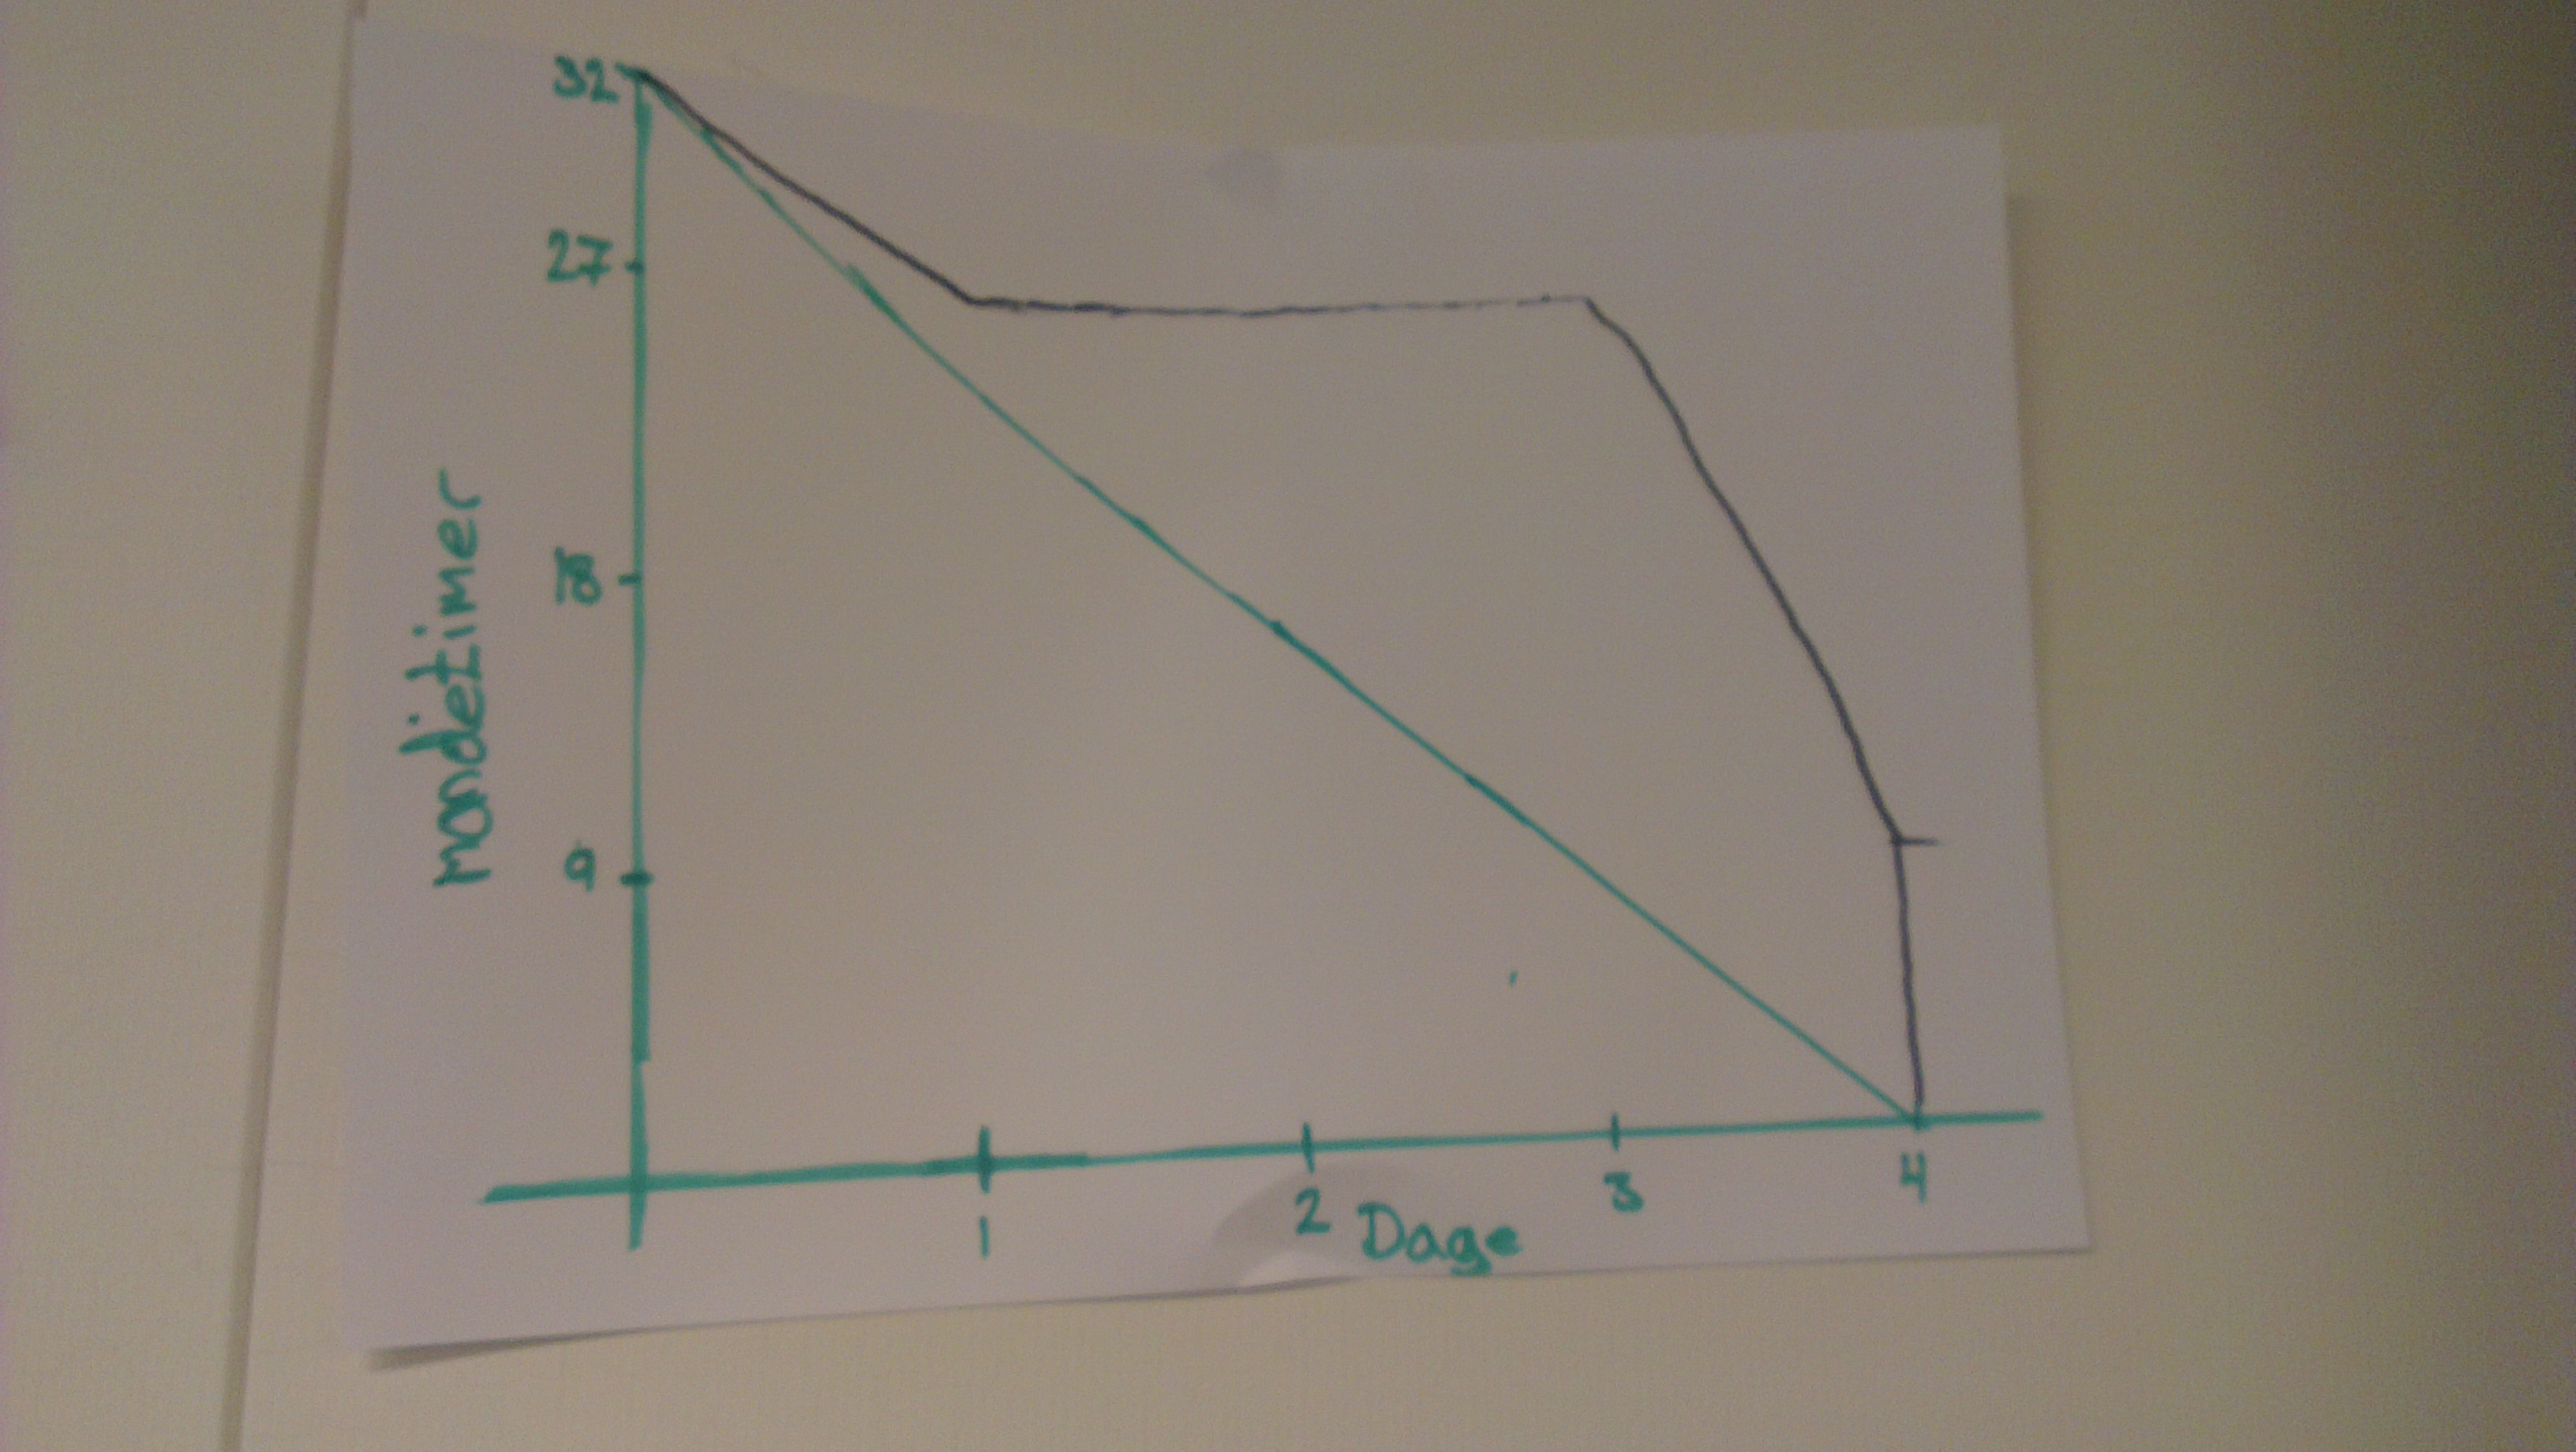
\includegraphics[scale=0.10]{includes/billeder/sprint2.jpg}
\subsubsection*{Product backlog}
Backlog lavet den 9.12.2013 i starten af sprint 2. \\
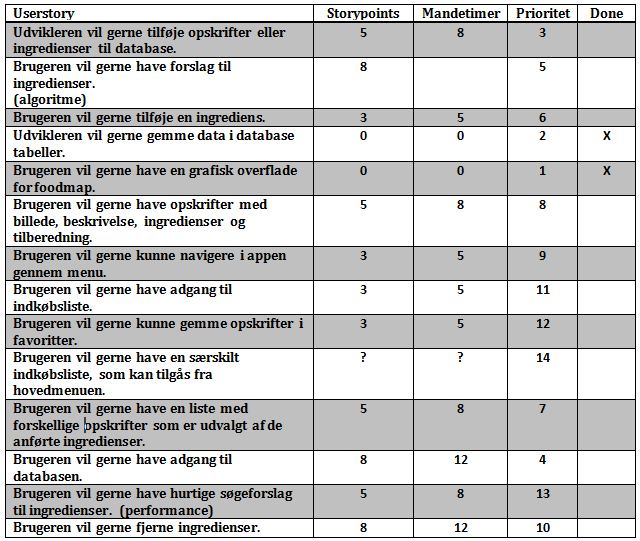
\includegraphics[scale=0.60]{includes/billeder/productbacklog_sprint2.png}

\subsubsection*{Sprint backlog}
I sprint 2 fokuserede vi p� f�lgende user stories: \\
Database kobling, dummy data til databasen, algoritme. \\
Samt database tabeller og basic gui som vi satte til 0 mandetimer, eftersom de var f�rdige efter at have opdelt dem, da de var for store. 

\subsection*{Xp og scrum praktikker}
I sprint 2 benyttede vi XP praktikkerne: stand-up meeting, planning poker, par programmering, kollektivt kode ejerskab, refactoring, kodestandarder, metafor og simpelt design. \\
Vi havde en scrum master, men product owner droppede vi, da det ikke giver s� meget mening i en gruppe af 3.

\subsection*{Produkt review}
Til produkt reviewet var det planen at vi ville vise vores gui med database adgang, men Android emuleratoren fejlede og pr�sentationen faldt derfor til bunden. Det endte med at vi kun viste selve databasen med data. 


\subsection*{Retrospektive}
I sprint 2 blev vi endeligt f�rdige med b�de databasen og koblingen mellem database og gui, dog f�rst efter at have en del overarbejde. Samtidigt havde vi overvurderet hvor mange ressourcer vi egentligt havde til r�dighed og n�ede derfor at br�nde 20 ud af 32 mandetimer.

\subsubsection*{Hvad gik godt}
Sprint 2 gik meget bedre end sprint 1 idet at vi endeligt fik styr p� database delen af vores projekt, dog efter meget overarbejde. Samtidigt fik vi en positiv oplevelse af at f� opsplittet vores user stories bedre, da de dermed blev mere pr�cise b�de i formulering og estimering. 

\subsubsection*{Hvad gik mindre godt}
Vi skulle have v�ret lidt bedre forberedt til produkt reviewet; det kunne m�ske have v�ret muligt at undg� problemer med emulatoren og kunden havde f�et et bedre indtryk af hvad vi havde lavet.

\subsubsection*{Hvad �ndrer vi til n�ste sprint}
En revurdering af vores velocity, da vi �benlyst havde vurderet den for h�jt igen og m�tte s�ge at lave et mere overkommeligt m�l.

\newpage

\subsection*{Sprint 3}
\subsection*{Velocity}
Lav velocity blah blah...

\subsection*{Planl�gning}

\subsubsection*{Product backlog}
Til product backloggen har vi i dette sprint tilf�jet en userstory med unit testing, samt at vi har �ndret prioriteten for diverse stories. \\
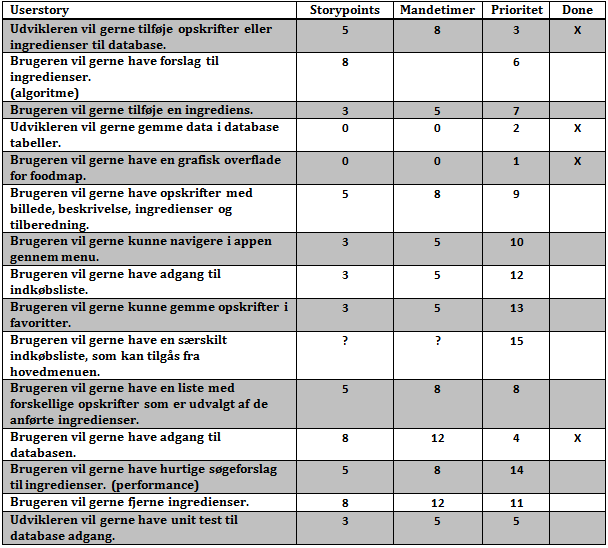
\includegraphics[scale=0.70]{includes/billeder/productbacklog_sprint3.png}

\subsubsection*{Sprint backlog}
I sprint backloggen for dette sprint indg�r de to userstories: \\
\begin{itemize}
\item Udvikleren vil gerne have unit test til database adgang.
\item Brugeren vil gerne have forslag til ingredienser. (algoritme)
\end{itemize}

Ud af disse to stories fik vi lavet unit testene.

\subsection*{Xp og scrum praktikker}
I sprint 3 benyttede vi fortsat XP praktikkerne: stand-up meeting, planning poker, par programmering, kollektivt kode ejerskab, kodestandarder, story board, metafor og simpelt design.

\subsection*{Produkt review}
Til reviewet viste vi vores foodmap gui med den funktionalitet vi havde n�et, samt vores unit test.

\subsubsection*{Konklusion af review}
N�ede kun unit testing.

\subsection*{Retrospektive}
Godt: \\
Vi fik lavet unit test og dermed fik vi lidt mere kvalitetssikring ind over vores projekt. \\

Kunne have v�ret bedre: \\
Alt for kort sprint med de 3 mandedage og derfor for meget pres p� for at have noget klar til reviewet. Is�r iforhold til at have noget visuelt klar at kunne vise. \\
Vi havde lidt meget parprogrammering pga. vores fokus p� test. 

Hvad �ndrer vi til n�ste sprint: \\
Vi var sprint 3 det sidste sprint, men ellers havde vi prim�rt fors�ge at lave et l�ngere sprint hvor vi arbejdede lidt mere spredt.


\section*{Konklusion p� sprints}
Vores sprints var for korte og der var for meget stress p� i forhold til at have noget klar til hvert review. \\
hvad har v�ret godt og d�rligt i sprintsene...


\part{Konklusion}


\subsection*{Future works}

\newpage
\part{Bibliografi}
\bibliography{bibliografi}
\bibliographystyle{plain}
\appendix

\newpage
\part{Appendix}
\input{appendix.tex}

\end{document}